\documentclass[12pt]{article}

\usepackage[a4paper,left=25mm,right=25mm,top=35mm,bottom=25mm]{geometry}
\usepackage{ngerman}
\usepackage{parskip}
\usepackage{times}
\usepackage{graphicx}
\usepackage{listings}
\usepackage{fancyhdr}

\setlength{\headheight}{15.2pt}
\pagestyle{fancy}

\lhead{Bildverarbeitung und Mustererkennung\\Praktikum Blatt 1}
\rhead{Patrick Hüntelmann\\22.04.2022}

\lstset{
  basicstyle=\ttfamily,
  breakatwhitespace=false,         % sets if automatic breaks should only happen at whitespace
  breaklines=true,                 % sets automatic line breaking
  captionpos=b,                    % sets the caption-position to bottom
  deletekeywords={...},            % if you want to delete keywords from the given language
  escapeinside={\%*}{*)},          % if you want to add LaTeX within your code
  extendedchars=true,              % lets you use non-ASCII characters; for 8-bits encodings only, does not work with UTF-8
  frame=single,	                   % adds a frame around the code
  keepspaces=true,                 % keeps spaces in text, useful for keeping indentation of code (possibly needs columns=flexible)
  language=python,                 % the language of the code
  showstringspaces=false,          % underline spaces within strings only
  showtabs=false,                  % show tabs within strings adding particular underscores
  tabsize=2,	                   % sets default tabsize to 2 spaces
}

\begin{document}

\pagenumbering{arabic}

\section*{Aufgabe 1}
\subsection*{a) Farben benennen}
Welche Farben befinden sich an den folgenden Koordinaten

(0,0,0): Schwarz\\
(1,0,0): Rot\\
(0,1,0): Grün\\
(0,0,1): Blau\\
(1,1,0): Gelb\\
(1,0,1): Magenta\\
(0,1,1): Cyan\\
(0.6,0.6,0.6): Grau

\newpage

\subsection*{b) Schattenerkennung}
\subsubsection*{1. Konvertierung in das YUV-Format}
Die Konvertierung einer RGB-Farbe in das YUV-Format ist in der Funktion \textbf{rgb\_to\_yuv} (main.py Zeile 5) implementiert. Diese Funktion bekommt die RGB-Farbe über die Parameter übergeben und gibt einen Tupel zurück, welche eine identische Farbe im YUV-Format darstellt.

\begin{tabular}{c | c | c}
  Y-Kanal & U-Kanal & V-Kanal \\
  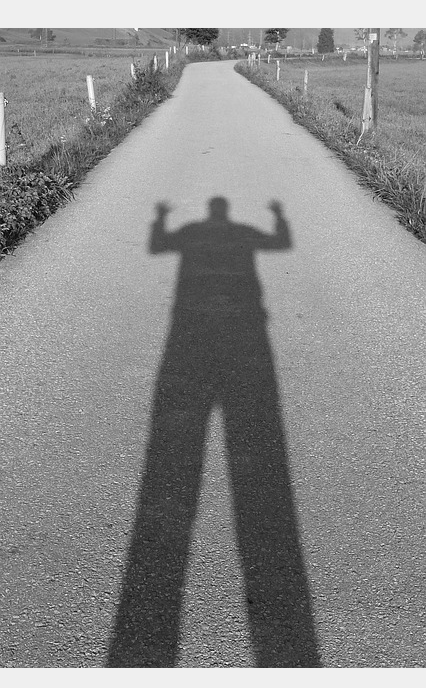
\includegraphics[width=.3\linewidth]{y.png} & 
\includegraphics[width=.3\linewidth]{u.png} & 
\includegraphics[width=.3\linewidth]{v.png}
\end{tabular}

\subsubsection*{2. Schattenregion bestimmen}
Die Erzeugung der Ergebnisbilder T\textsubscript{1} und T\textsubscript{2} wurde in der Funktion \textbf{threshold} (main.py Zeile 26) implementiert. Diese Funktion bekommt den entsprechenden Kanal (U für T\textsubscript{1}, V für T\textsubscript{2}) übergeben und gibt das Ergebnisbild zurück, welches innerhalb der Funktion berechnet wurde.
\begin{tabular}{c | c | c}
  T\textsubscript{1} & T\textsubscript{2} & Schattenregion \\
  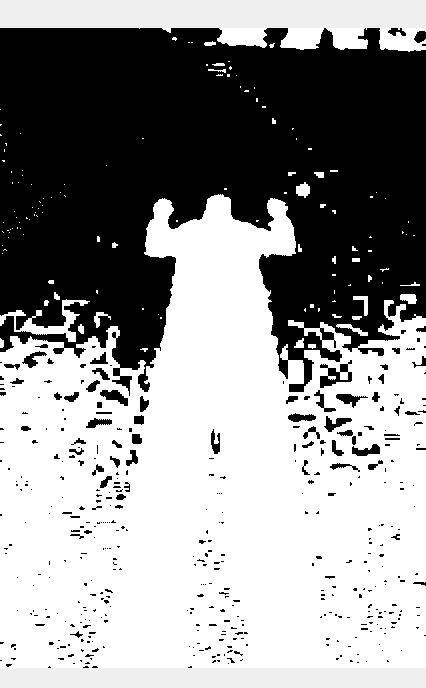
\includegraphics[width=.3\linewidth]{t1.png} & 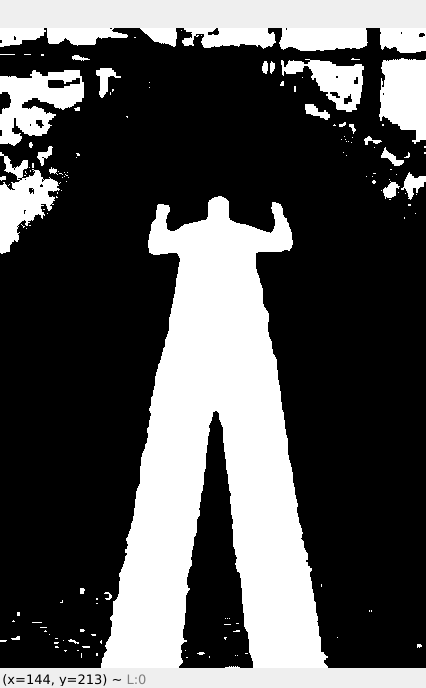
\includegraphics[width=.3\linewidth]{t2.png} & 
\includegraphics[width=.3\linewidth]{s.png}
\end{tabular}

\end{document}
